\subsubsection{Motivation for RNN tagging}

Within the decay of a $b$-hadron, several charged particles can emerge from the secondary (or tertiary) decay vertex with large impact parameters, as measured by the distance of closest approach to the primary vertex. These impact parameters are intrinsically correlated: if one track is found with a large impact parameter then finding a second track with large impact parameter is more likely. If no secondary vertex is present, as in light-flavor jets, then such a correlation should not exist. The 2D distribution of transverse impact parameter significance\footnote{In all algorithms discussed here the impact parameter is characterized by the lifetime signed transverse impact parameter significance ($\sdip \equiv d_0 / \sigma_{d_0}$) and the lifetime signed longitudinal impact parameter significance ($\szip \equiv z_0 \sin \theta / \sigma_{z_0 \sin \theta}$).} (\sdip) for the leading and subleading transverse impact parameter significance tracks can be found in Figure~\ref{fig:ip_corr} for $b$-jets, where a correlation can clearly be seen, and light flavour-jets, where no such correlation is observed.
\begin{figure}[htbp]
  \centering
   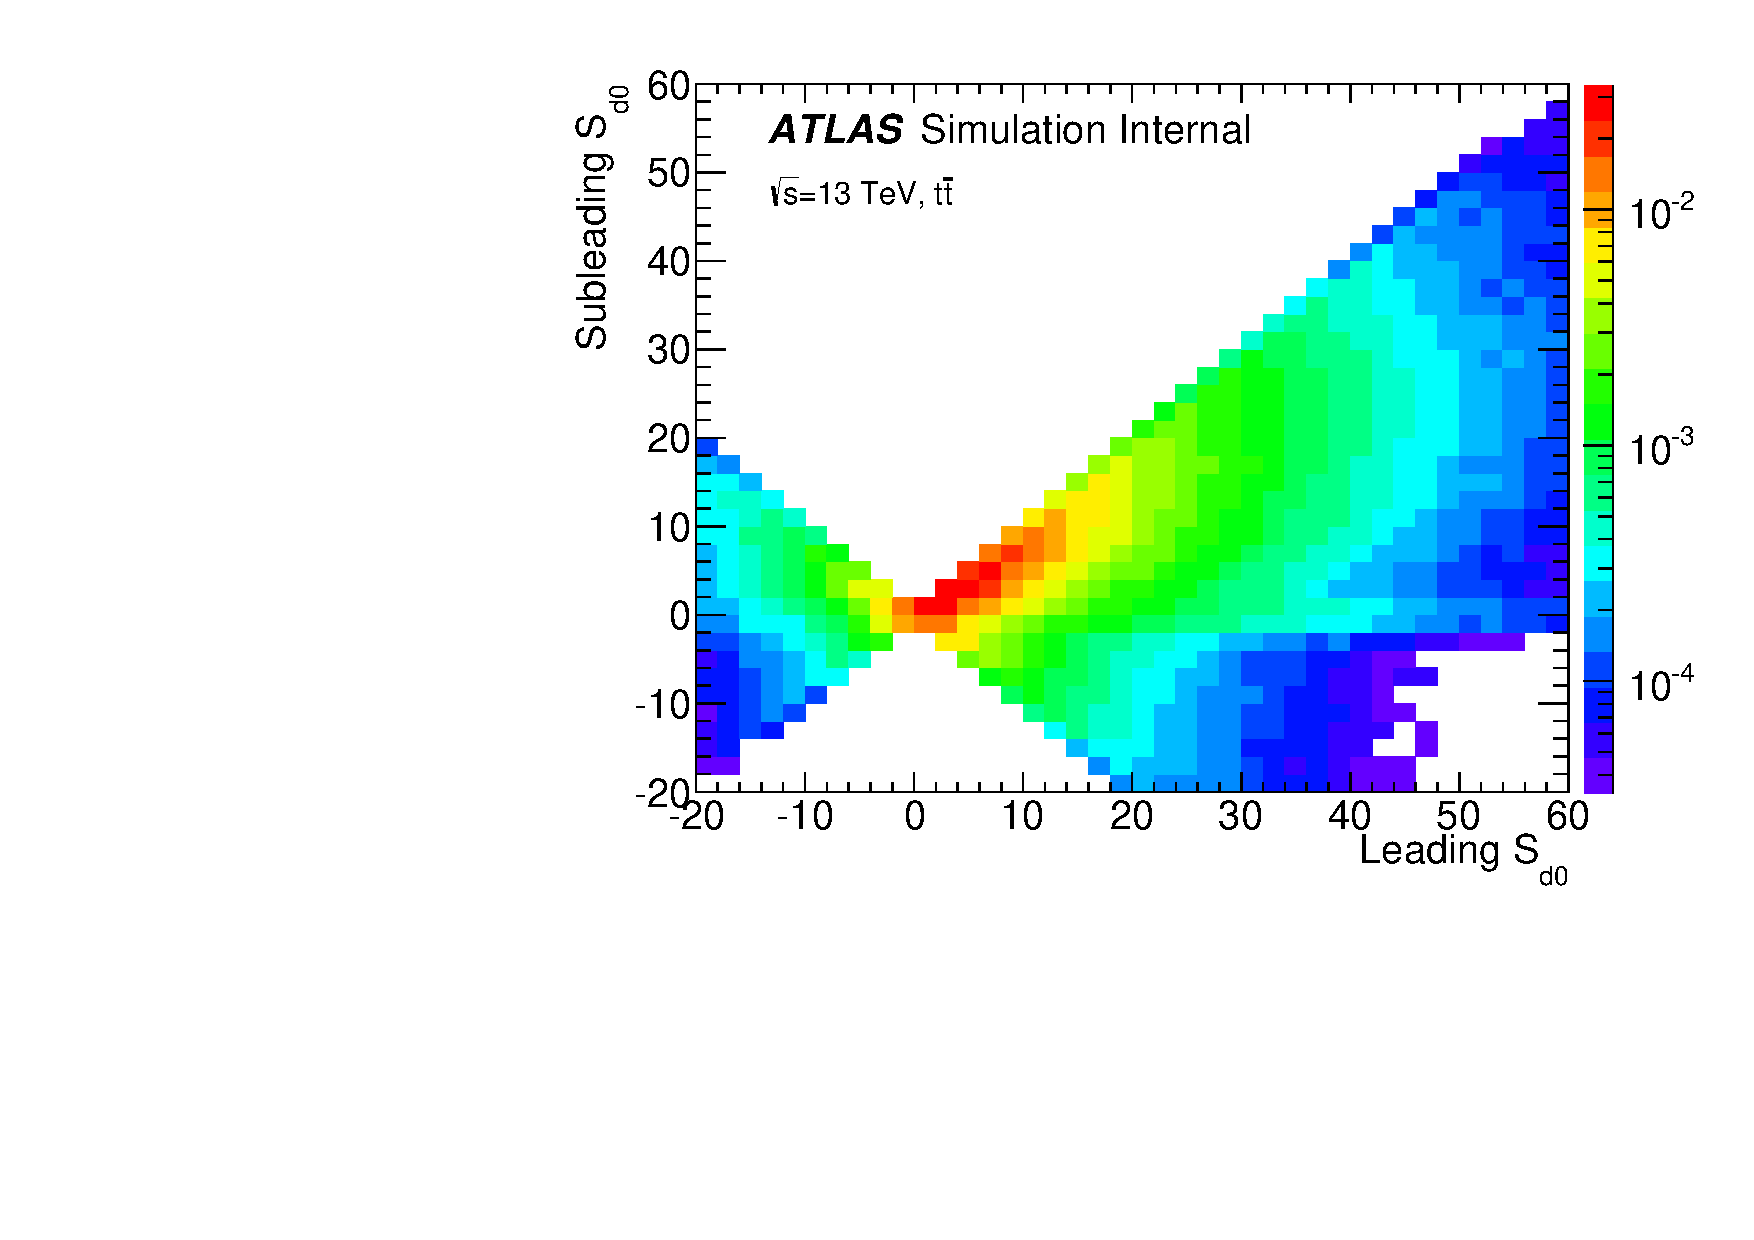
\includegraphics[width=0.48\textwidth]{figures/RNN/Sd0_2d_B.pdf}
 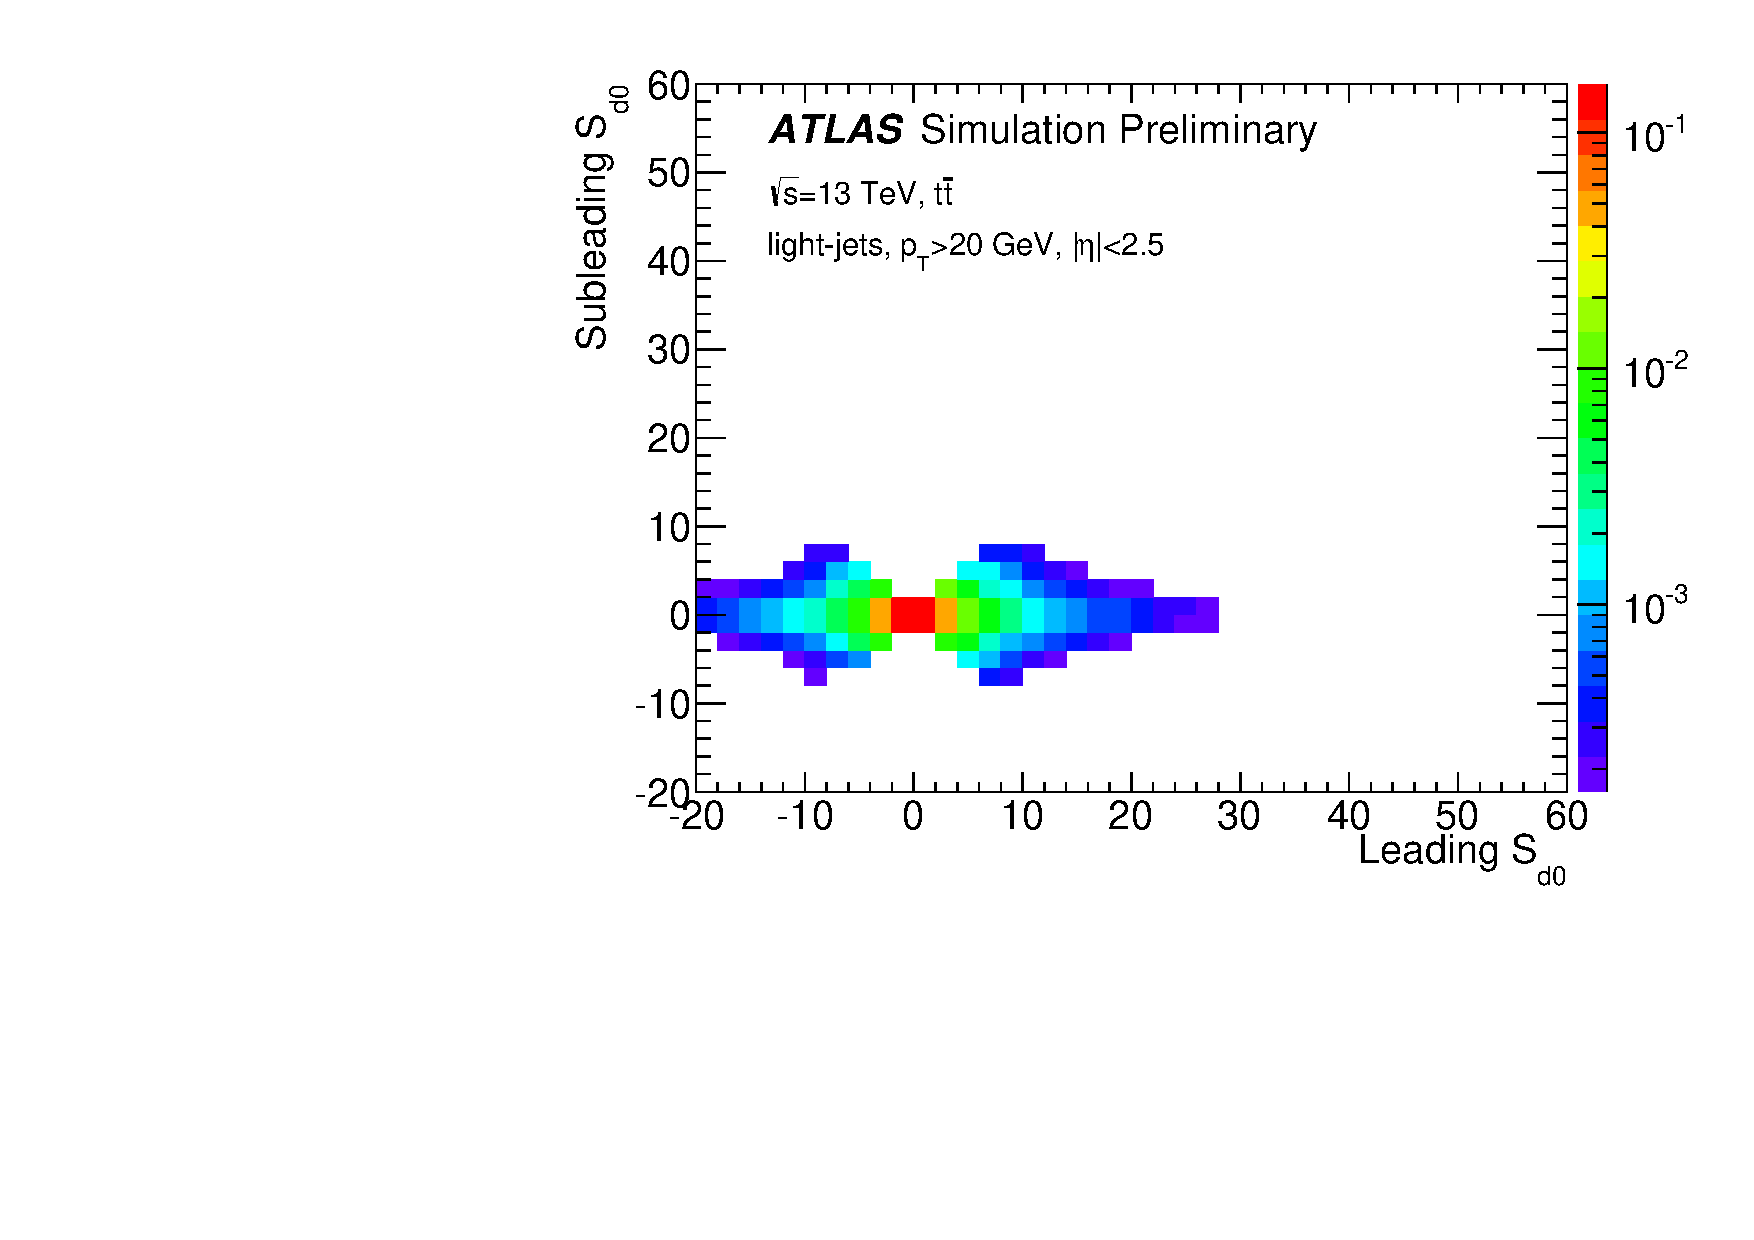
\includegraphics[width=0.48\textwidth]{figures/RNN/Sd0_2d_L.pdf}
\caption{The distribution of the $d_0$ significance for the leading $d_0$ significance and subleading $d_0$ significance track in $b$-jets (left) and light jets (right). }
  \label{fig:ip_corr}
\end{figure}


ATLAS's baseline IP based $b$-tagging algorithm, IP3D, uses 3D likelihood templates in $\sdip$, $\szip$, and a track categorization to compute three per-flavor conditional likelihoods, $p_b$, $p_c$, and $p_{\textrm{light}}$. These likelihood templates are derived from histograms with 35 bins in $\sdip$, 20 bins in $\szip$, and 14 bins in track category, where each category corresponds to a different track quality~\cite{ATL-PHYS-PUB-2015-022}. Multiplying by the three flavors, this results in a final bin count of $35 \times 20 \times 14 \times 3 = 29,400$. As the probability is computed per track, the likelihood of a jet being of a given flavour is computed as the product of the per-track likelihoods. The IP3D discriminant is built from the conditional log-likelihood ratio, $\textrm{IP3D}=\ln \prod_{i \in \textrm{tracks}} p_b^i / p_{\textrm{light}}^i$.

One of the main assumptions of the IP3D algorithm is that the per-track flavor conditional likelihood can be computed independent of the other tracks in the jet.  Such a likelihood model does not take into account correlations amongst track parameters, and the method of building templates to define likelihoods requires large sample sizes. 
In addition, extending the template to account for additional kinematic variables is computationally expensive, since the number of template bins (and the number of simulated events required to fill them) grows exponentially with the number of variables.
Such deficiencies of the algorithm can be rectified using machine learning classifiers.


\subsubsection{Recurrent Networks}

Recurrent neural networks are used to directly learn sequence-based dependencies for arbitrary-length inputs with strong ordering~\cite{ref:RNNthesis, dlbook}. The fundamental unit of an RNN is a cell encapsulating an internal state vector. As the first step of processing any given sequence (in this case the tracks in a jet), the internal state is initialized to zero. At each step in the sequence, the cell is handed a fixed number of inputs (in this case the parameters that describe one track). These parameters are combined with the \emph{current} internal state in order to compute a \emph{new} internal state based on a set of rules which are tuned in the training phase. At the end of the sequence the cell's internal state serves as a fixed-dimensional representation of the entire sequence. In this way a recurrent cell is able to reduce a sequence of arbitrary length to a fixed number of variables, which can then be processed by a traditional feed-forward network.\footnote{For a review of terminology such as ``feed-forward'', ``fully-connected'', and ``softmax'' and a more pedagogical introduction to deep learning, see for instance ~\cite{dlbook,2014arXiv1404.7828S}.}

Much of the recent success of RNNs in various natural language and long-sequence processing applications can be attributed to the advent of Long Short-Term Memory (LSTM)~\cite{ref:LSTM} units and later variants such as Gated Recurrent Units (GRUs)~\cite{ref:GRU,cho14}. These architectural modifications at the cell level mitigate issues related to vanishing and exploding gradients~\cite{hochreiter1991untersuchungen,Bengio:1994:LLD:2325857.2328340,DBLP:journals/corr/abs-1211-5063}, and improve the knowledge persistence of long-term dependencies. These special kinds of recurrent units employ different internal gating mechanisms to modify the cell state in order to balance and regulate the relative importance of long-term and short-term information.
